%-----------------------------------------------------------------------------%
\chapter{\babDua}
%-----------------------------------------------------------------------------%
Bab ini berisi dasar-dasar pemahaman yang diperlukan dalam membuat program logika. 
%-----------------------------------------------------------------------------%
\section{Pendahuluan}
Diberikan himpunan alfabet \( \mathcal{A} \) dari bahasa \( \mathcal{L} \), akan didefinisikan himpunan berhingga yang saling \f{disjoint} yaitu himpunan konstanta, himpunan simbol fungsi, dan himpunan simbol predikat. Selain itu, pada alfabet juga mengandung himpunan simbol variabel. Simbol \f{underscore} (\_) dikhususkan untuk menyatakan sebuah \f{anonymous} variabel. \f{Term} dari \( \mathcal{A} \) didefinisikan secara rekursif sebagai salah satu dari: variabel, konstanta, atau ekspresi dengan bentuk \f{f(t$_{1}$,...,t$_{n}$)} dengan \f{f} adalah simbol fungsi dari \( \mathcal{A} \) dan \f{t$_{i}$} adalah term. \f{Atom} dari \( \mathcal{A} \) adalah ekspresi dengan bentuk \f{p(t$_{1}$,...,t$_{n}$)} dengan \f{p} adalah simbol predikat dari \( \mathcal{A} \) dan \f{t$_{i}$} adalah term. Selanjutnya, notasi \f{p/n} digunakan untuk menyatakan predikat \f{p} memiliki arity \f{n}. \f{Literal} adalah sebuah atom \f{a} atau negasinya \f{not a}. Literal \f{not a} (seperti pada bentuk kedua) disebut \f{default} literal. Sebuah term (atom maupun literal) disebut \f{ground} jika term tersebut tidak memiliki variabel. Himpunan seluruh ground term dari \( \mathcal{A} \) disebut Herbrand Universe dari \( \mathcal{A} \).
\section{Program Logika}\label{cha:kompar}
%-----------------------------------------------------------------------------%
Program logika adalah himpunan berhingga dari \f{rule} dengan bentuk:
\begin{displaymath}
	H \leftarrow L_1,...,L_n
\end{displaymath}
dengan \f{H} adalah sebuah \f{atom}, $m \geq 0$, dan $L_i$ adalah \f{literal}. \f{H} dan $L_i$ berturut-turut disebut sebagai \f{head} dan \f{body} dari sebuah rule.

Operator koma pada sebuah rule dibaca sebagai konjungsi. Sebuah program logika disebut \f{definit} jika pada program logika tersebut tidak mengandung default literal. Rule yang tidak memiliki body ditulis sebagai $H$ saja, alih-alih menuliskannya sebagai $H \leftarrow $ . Rule dengan bentuk seperti ini disebut sebagai sebuah \f{fakta}.
%-----------------------------------------------------------------------------%
\subsection{Pengertian X}
%-----------------------------------------------------------------------------%
Setiap gambar dapat diberikan caption dan diberikan label. Label dapat digunakan untuk menunjuk gambar tertentu. Jika posisi gambar berubah, maka nomor gambar juga akan diubah secara 
otomatis. Begitu juga dengan seluruh referensi yang menunjuk pada gambar tersebut.

Contoh sederhana adalah \pic~\ref{fig:exmasalahparalel}. Silahkan lihat code \latex~dengan nama bab2-landasan-teori.tex untuk melihat kode lengkapnya. Harap diingat bahwa caption untuk gambar selalu terletak dibawah gambar.
Dibawah adda figure, jangn lupa dimention dengan \ref{fig:exmasalahparalel}. 

\begin{figure}
	\centering
	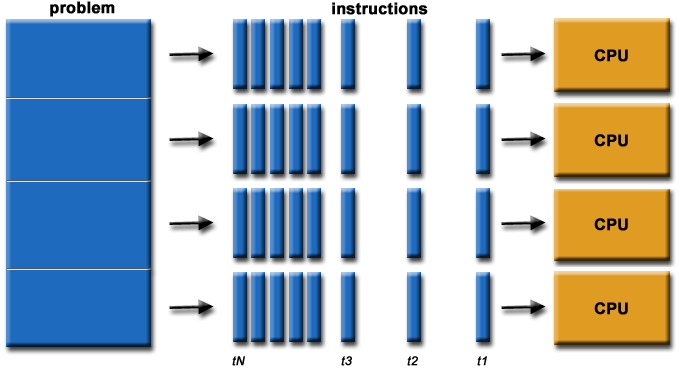
\includegraphics[width=0.8\textwidth]
		{pics/parallelProblem.png}
	\caption{Contoh masalah yang dikerjakan secara paralel}
	\label{fig:exmasalahparalel}
\end{figure}
\vspace{-0.8cm}
\begin{center}
{\small Sumber gambar: \citep{net.oxford}}
\end{center}

%-----------------------------------------------------------------------------%
\subsection{Klasifikasi X}
%-----------------------------------------------------------------------------%
Figure dalam enum dan dua sitasi sekaligus \citep{book.buyya,book.sterling-jones} :  
\begin{enumerate}
\item \bi{Bold Italic} \\
Penjelasan....... Untuk gambarannya dapat dilihat di Gambar \ref{fig:neumann}.

\begin{figure}
	\centering
	\includegraphics[height=0.65\textwidth,width=0.6\textwidth]
		{pics/neumann.pdf}
	\caption{Arsitektur klasik \f{von Neumann}}
	\label{fig:neumann}
\end{figure}
\vspace{-1.2cm}
\begin{center}
{\small Sumber gambar terinspirasi dari: \citep{buku.pressman}}
\end{center} 

\item \bi{Sesuatu banget} \\
Penjelasan.......
\end{enumerate}
\paragraph{}
%-----------------------------------------------------------------------------%
\section{\f{Section in Eng}}
%-----------------------------------------------------------------------------%
Hal pertama yang mungkin ditanyakan adalah bagaimana membuat huruf tercetak tebal, miring, atau memiliki garis bawah. 
Pada Texmaker, Anda bisa melakukan hal ini seperti halnya saat mengubah dokumen dengan LO Writer. 
Namun jika tetap masih tertarik dengan cara lain, ini dia: 

\begin{itemize}
	\item \bo{Bold} \\
		Gunakan perintah \bslash textbf$\lbrace\rbrace$ atau 
		\bslash bo$\lbrace\rbrace$. 
	\item \f{Italic} \\
		Gunakan perintah \bslash textit$\lbrace\rbrace$ atau 
		\bslash f$\lbrace\rbrace$. 
	\item \underline{Underline} \\
		Gunakan perintah \bslash underline$\lbrace\rbrace$.
	\item $\overline{Overline}$ \\
		Gunakan perintah \bslash overline. 
	\item $^{superscript}$ \\
		Gunakan perintah \bslash $\lbrace\rbrace$. 
	\item $_{subscript}$ \\
		Gunakan perintah \bslash \_$\lbrace\rbrace$. 
\end{itemize}

Perintah \bslash f dan \bslash bo hanya dapat digunakan jika package 
uithesis digunakan. 
%-----------------------------------------------------------------------------%
\subsection{Pengertian \f{Section in Eng}}
%-----------------------------------------------------------------------------%

%-----------------------------------------------------------------------------%
\subsection{Next Subsection \f{Section in Eng}}
%-----------------------------------------------------------------------------%

%-----------------------------------------------------------------------------%
\section{\f{Keatas lagi}}
%-----------------------------------------------------------------------------%
Contoh cite yang ga ada \cite{gaib}. Cite author \citeauthor{article.rebecca},cite tahun \citeyear{article.treese}, cite mention \cite{adin.experiment}, dan cite di akhir kalimat \citep{techreport.nist}.
%-----------------------------------------------------------------------------%
\subsection{\f{Masuk lagi}}
%-----------------------------------------------------------------------------%
Footnote example nih : MPICH \footnote{\url{http://www.mpich.org/}}, LAM/MPI \footnote{\url{http://www.lam-mpi.org/}}, dan OpenMPI \footnote{\url{www.open-mpi.org}} \citep{article.mcguire}. MPI-3 sedang dalam tahap perencanaan \footnote{\url{http://meetings.mpi-forum.org/MPI_3.0_main_page.php}}. Fungsi-fungsi tersebut berada di tabel \ref{tab:mpifund}. (Contoh tabel).

\begin{table}
	\centering
	\caption{Fungsi fundamental MPI}
	\label{tab:mpifund}
	\begin{tabular}{|c|c|c|}
	\hline
	\rowcolor{headertbl}	
	\hline No. & Nama Fungsi & Penjelasan \\ 
	\hline 1 & MPI\_Init & Memulai kode MPI \\ 
	\hline 2 & MPI\_Finalize & Mengakhiri kode MPI \\ 
	\hline 3 & MPI\_Comm\_size & Menentukan jumlah proses \\ 
	\hline 4 & MPI\_Comm\_rank & Menentukan label proses \\ 
	\hline 5 & MPI\_Send & Mengirim pesan \\ 
	\hline 6 & MPI\_Recv & Menerima pesan \\ 
	\hline
	\end{tabular}
\end{table}
\begin{center}
{\small Sumber tabel: taro sitasi disini, if i were u}
\end{center}